\section{Popis jednotlivých součástek a důvody konkrétního tvaru}

\begin{wrapfigure}{R}[0.2\textwidth]{0.7\textwidth}
    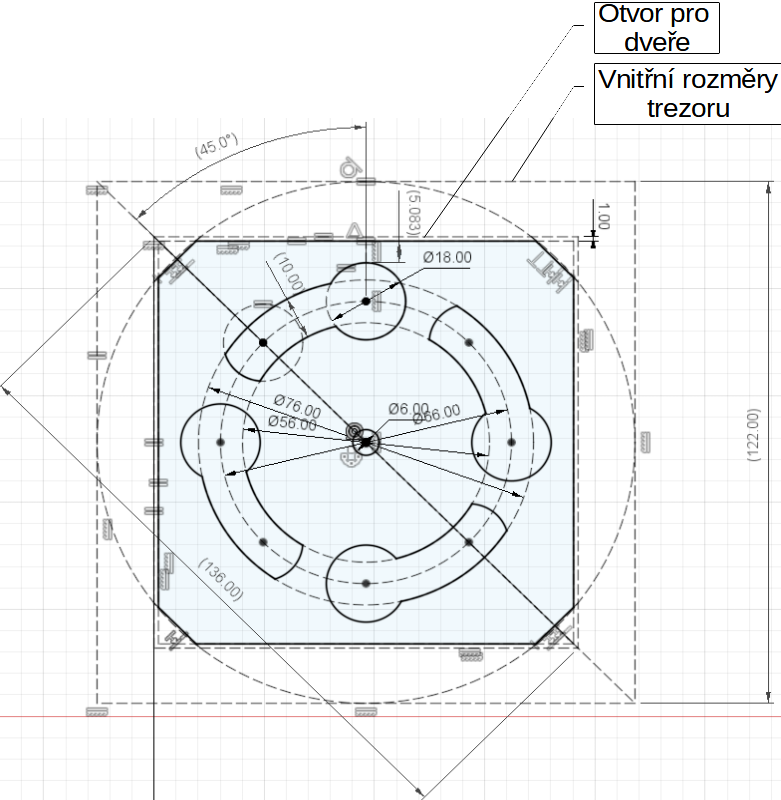
\includegraphics[width=0.7\textwidth]{kapitoly/obrazky/M3/geometrie_zapadky.png}
    \caption{náčrt} %todo čeho náčrt? 
    \label{fig:M3-geometrie-zapadky}
\end{wrapfigure} %todo zvážil bych obrázek centrovaný a obtékaný pouze nahoře a dole 

\subsection*{Geometrie západky}
Trezor má tvar krychle a~délku hrany má 128~mm, násobek šestnácti jsem zvolil kvůli jednoduché návaznosti na dřívka, %todo přidáme pár vět o dřívkách 
 dřevěná dřívka s obdélníkovým průřezem 3x16~mm nebo 2x16~mm. 
Protože je trezor vyroben z překližky o síle 4~mm, jsou jeho vnitřní rozměry o 4~mm na každé straně menší (takže 122~mm). 

%todo tady asi chybí další tvary? 